\subsection{Finetuning Analysis}
\label{sec:finetuning_analysis}

We investigate whether task-specific finetuning can improve GPS reasoning by comparing a finetuned Qwen3-30B model against its zero-shot baseline.

\paragraph{Finetuning Setup.}
We finetune Qwen3-30B-A3B-Instruct (a 30B-total, 3B-active MoE model) using LoRA \cite{hu2022lora} on the GPSBench training split. Training uses both the Pure GPS and Applied tracks with chain-of-thought reasoning included in the target outputs: each training example contains step-by-step reasoning followed by a final answer, encouraging the model to learn intermediate computation steps rather than shortcut to answers. We use the Tinker platform for distributed finetuning with the following hyperparameters: learning rate $2 \times 10^{-5}$ with linear decay, batch size 32, LoRA rank 64, maximum sequence length 16{,}384 tokens, and 2 training epochs. The low learning rate is chosen to mitigate catastrophic forgetting of pretrained knowledge. Training data consists of the standard 60\% train split (2{,}040 samples per task $\times$ 17 tasks = 34{,}680 total samples). Evaluation is performed on the 30\% held-out test split. The Missing Data Inference task is excluded from evaluation and reserved as a memorization probe (Section~\ref{sec:rq2_granularity_robustness}).

\paragraph{Overall Results.}
Table~\ref{tab:finetuning_overall} shows that finetuning improves overall performance (+1.5\%), with Pure GPS gaining (+4.3\%) while Applied slightly degrades ($-$1.6\%).

\begin{table}[htbp]
\centering
\caption{Overall finetuning results on Qwen3-30B.}
\label{tab:finetuning_overall}
\small
\begin{tabular}{lccc}
\toprule
\textbf{Track} & \textbf{Zero-shot} & \textbf{Finetuned} & \textbf{$\Delta$} \\
\midrule
Applied & 52.3\% & 50.7\% & \textcolor{red}{$-$1.6\%} \\
Pure GPS & 53.1\% & 57.4\% & \textcolor{green!60!black}{+4.3\%} \\
\midrule
\textit{Combined} & \textit{52.7\%} & \textit{54.2\%} & \textit{\textcolor{green!60!black}{+1.5\%}} \\
\bottomrule
\end{tabular}
\end{table}

\begin{figure}[htbp]
\centering
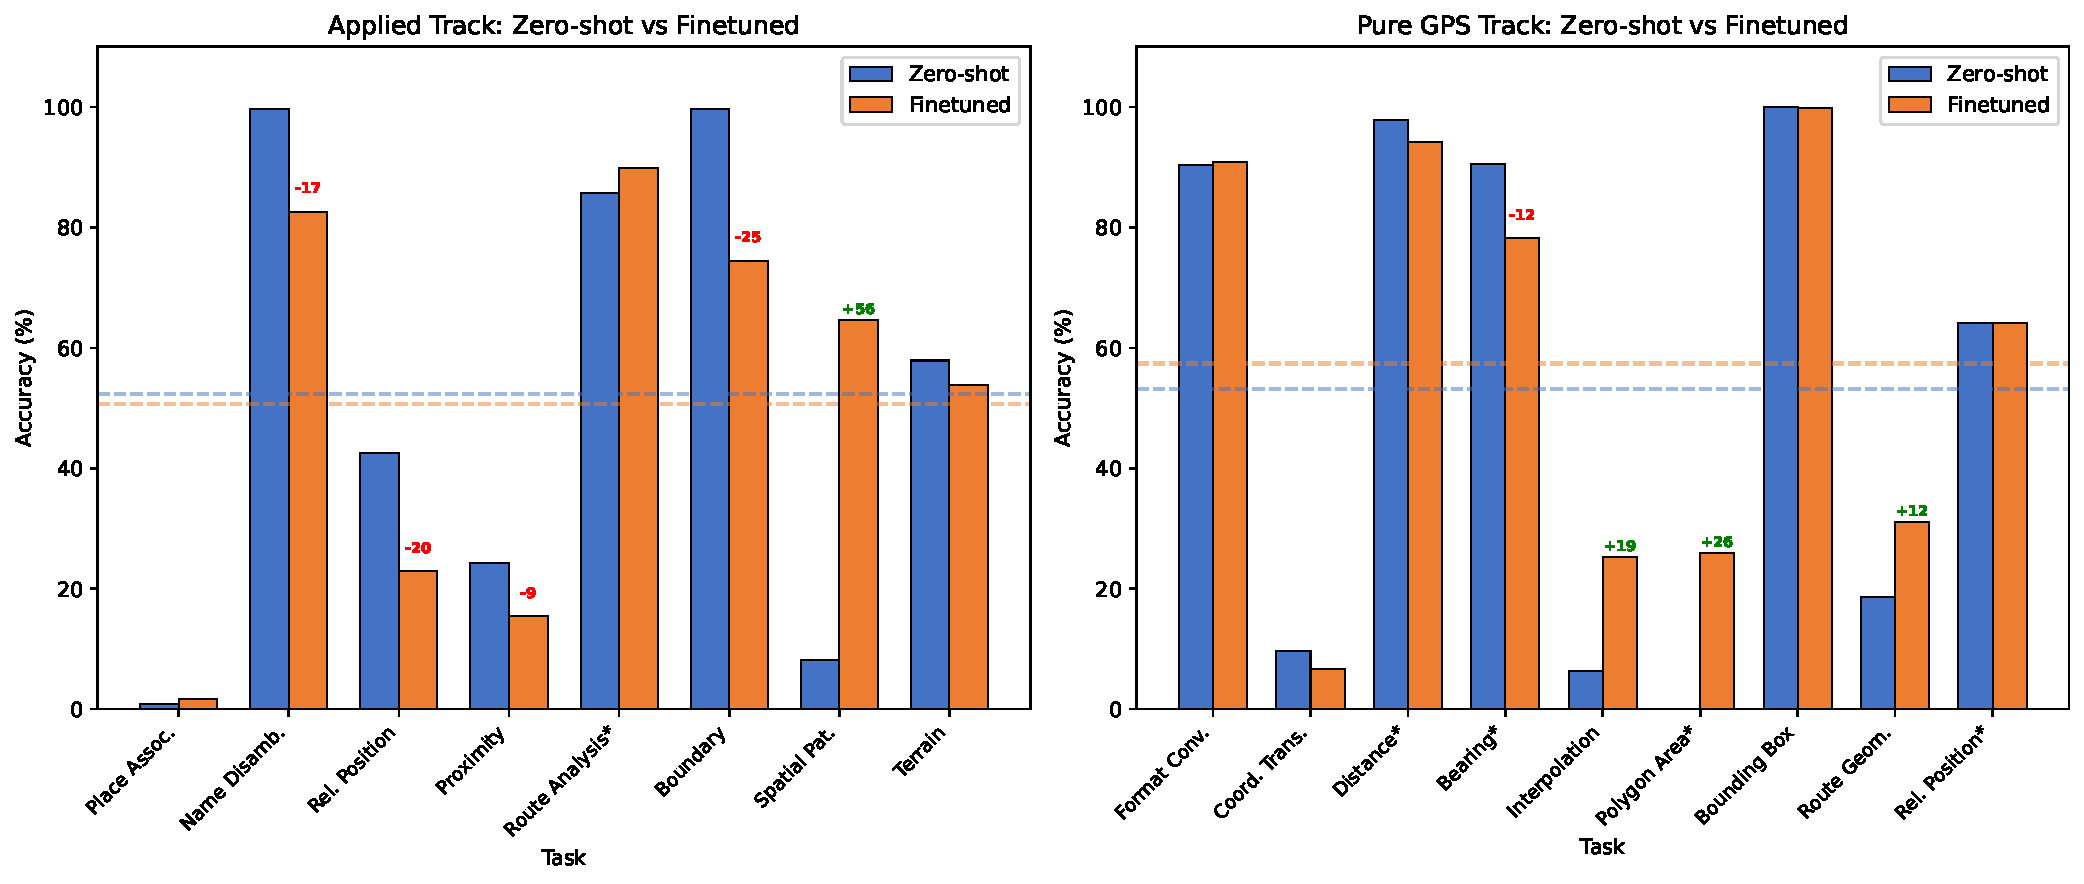
\includegraphics[width=\columnwidth]{figures/finetuning_comparison.pdf}
\caption{Zero-shot vs.\ finetuned performance on Qwen3-30B. Finetuning improves geometric tasks but degrades world knowledge integration.}
\label{fig:finetuning_comparison}
\end{figure}

\begin{table}[htbp]
\centering
\caption{Per-task finetuning comparison on Qwen3-30B. Green: improvement ($>$5\%), red: degradation ($<-$5\%).}
\label{tab:finetuning_comparison}
\small
\begin{tabular}{lccc}
\toprule
\textbf{Task} & \textbf{Zero-shot} & \textbf{Finetuned} & \textbf{$\Delta$} \\
\midrule
\multicolumn{4}{c}{\textit{Applied Track}} \\
\midrule
Place Association & 0.8 & 1.7 & \textcolor{gray}{+0.9} \\
Name Disambiguation & 99.7 & 82.6 & \textcolor{red}{$-$17.1} \\
Relative Position & 42.5 & 22.9 & \textcolor{red}{$-$19.6} \\
Proximity & 24.2 & 15.4 & \textcolor{red}{$-$8.8} \\
Route Analysis & 85.7 & 89.9 & \textcolor{gray}{+4.2} \\
Boundary Analysis & 99.7 & 74.5 & \textcolor{red}{$-$25.2} \\
Spatial Patterns & 8.1 & 64.6 & \textcolor{green!60!black}{+56.5} \\
Terrain & 57.9 & 53.9 & \textcolor{gray}{$-$4.0} \\
\midrule
\textit{Applied Overall} & \textit{52.3} & \textit{50.7} & \textit{\textcolor{red}{$-$1.6}} \\
\midrule
\multicolumn{4}{c}{\textit{Pure GPS Track}} \\
\midrule
Format Conversion & 90.4 & 90.9 & \textcolor{gray}{+0.5} \\
Coord.\ Transform & 9.7 & 6.6 & \textcolor{gray}{$-$3.1} \\
Distance & 97.8 & 94.2 & \textcolor{gray}{$-$3.6} \\
Bearing & 90.5 & 78.2 & \textcolor{red}{$-$12.3} \\
Interpolation & 6.4 & 25.3 & \textcolor{green!60!black}{+18.9} \\
Polygon Area & 0.0 & 25.9 & \textcolor{green!60!black}{+25.9} \\
Bounding Box & 100.0 & 99.9 & \textcolor{gray}{$-$0.1} \\
Route Geometry & 18.7 & 31.1 & \textcolor{green!60!black}{+12.4} \\
Relative Position$^\dagger$ & 64.1 & 64.1 & \textcolor{gray}{0.0} \\
\midrule
\textit{Pure GPS Overall} & \textit{53.1} & \textit{57.4} & \textit{\textcolor{green!60!black}{+4.3}} \\
\bottomrule
\multicolumn{4}{l}{\footnotesize $^\dagger$Format mismatch; assumed preserved.}
\end{tabular}
\end{table}

\paragraph{Task-Level Analysis.}
Table~\ref{tab:finetuning_comparison} reveals a clear pattern:

\textbf{Improvements}: Geometric reasoning tasks show significant gains---Spatial Patterns (+56.5\%), Polygon Area (+25.9\%), Interpolation (+18.9\%), and Route Geometry (+12.4\%).

\textbf{Degradation}: Tasks requiring world knowledge suffer---Boundary Analysis ($-$25.2\%), Relative Position ($-$19.6\%), and Name Disambiguation ($-$17.1\%). Bearing also degrades ($-$12.3\%).

\textbf{Preserved}: Format Conversion, Distance, and Bounding Box remain stable.

\paragraph{Finding.}
The pattern suggests finetuning enhances pure geometric computation while disrupting the model's integration of world knowledge. Boundary Analysis needs knowledge of administrative regions; Name Disambiguation relies on geographic entity understanding. These capabilities degrade while mathematically-grounded tasks improve.

\paragraph{Implications.}
Naive finetuning leads to capability trade-offs between geometric reasoning and world knowledge. Future work should explore multi-task balancing and continual learning techniques to preserve base capabilities while adding GPS skills.

